\chapter*{Заключение}                       % Заголовок
\addcontentsline{toc}{chapter}{Заключение}  % Добавляем его в оглавление

%% Согласно ГОСТ Р 7.0.11-2011:
%% 5.3.3 В заключении диссертации излагают итоги выполненного исследования, рекомендации, перспективы дальнейшей разработки темы.
%% 9.2.3 В заключении автореферата диссертации излагают итоги данного исследования, рекомендации и перспективы дальнейшей разработки темы.
%% Поэтому имеет смысл сделать эту часть общей и загрузить из одного файла в автореферат и в диссертацию:

Основные результаты работы заключаются в следующем.
%% Согласно ГОСТ Р 7.0.11-2011:
%% 5.3.3 В заключении диссертации излагают итоги выполненного исследования, рекомендации, перспективы дальнейшей разработки темы.
%% 9.2.3 В заключении автореферата диссертации излагают итоги данного исследования, рекомендации и перспективы дальнейшей разработки темы.
\begin{enumerate}
  \item На основе анализа предметной области был построен целый программно-аппаратный комплекс, выполняющий свою задачу;
  \item Тестирования показали, что робот, в большинстве случаев справляется со своей задачей нахождения целевых объектов;
  \item Моделирование различных ситуаций показало, что робот справится далеко не с каждым случаем, в котором он может оказаться (например, на широкой улице). Поэтому для конкретных случаев требуется дополнительное совершенствование и корректировка текущей реализации.
\end{enumerate}

Таким образом была разработана система управления и формирования поведенческой стратегии автономного мобильного робота на основе визуального анализа окружающего пространства. Изображения готового робота можно \fixme{увидеть на Рисунке }.

\begin{figure}[ht]
  \begin{minipage}[b][][b]{0.49\linewidth}\centering
    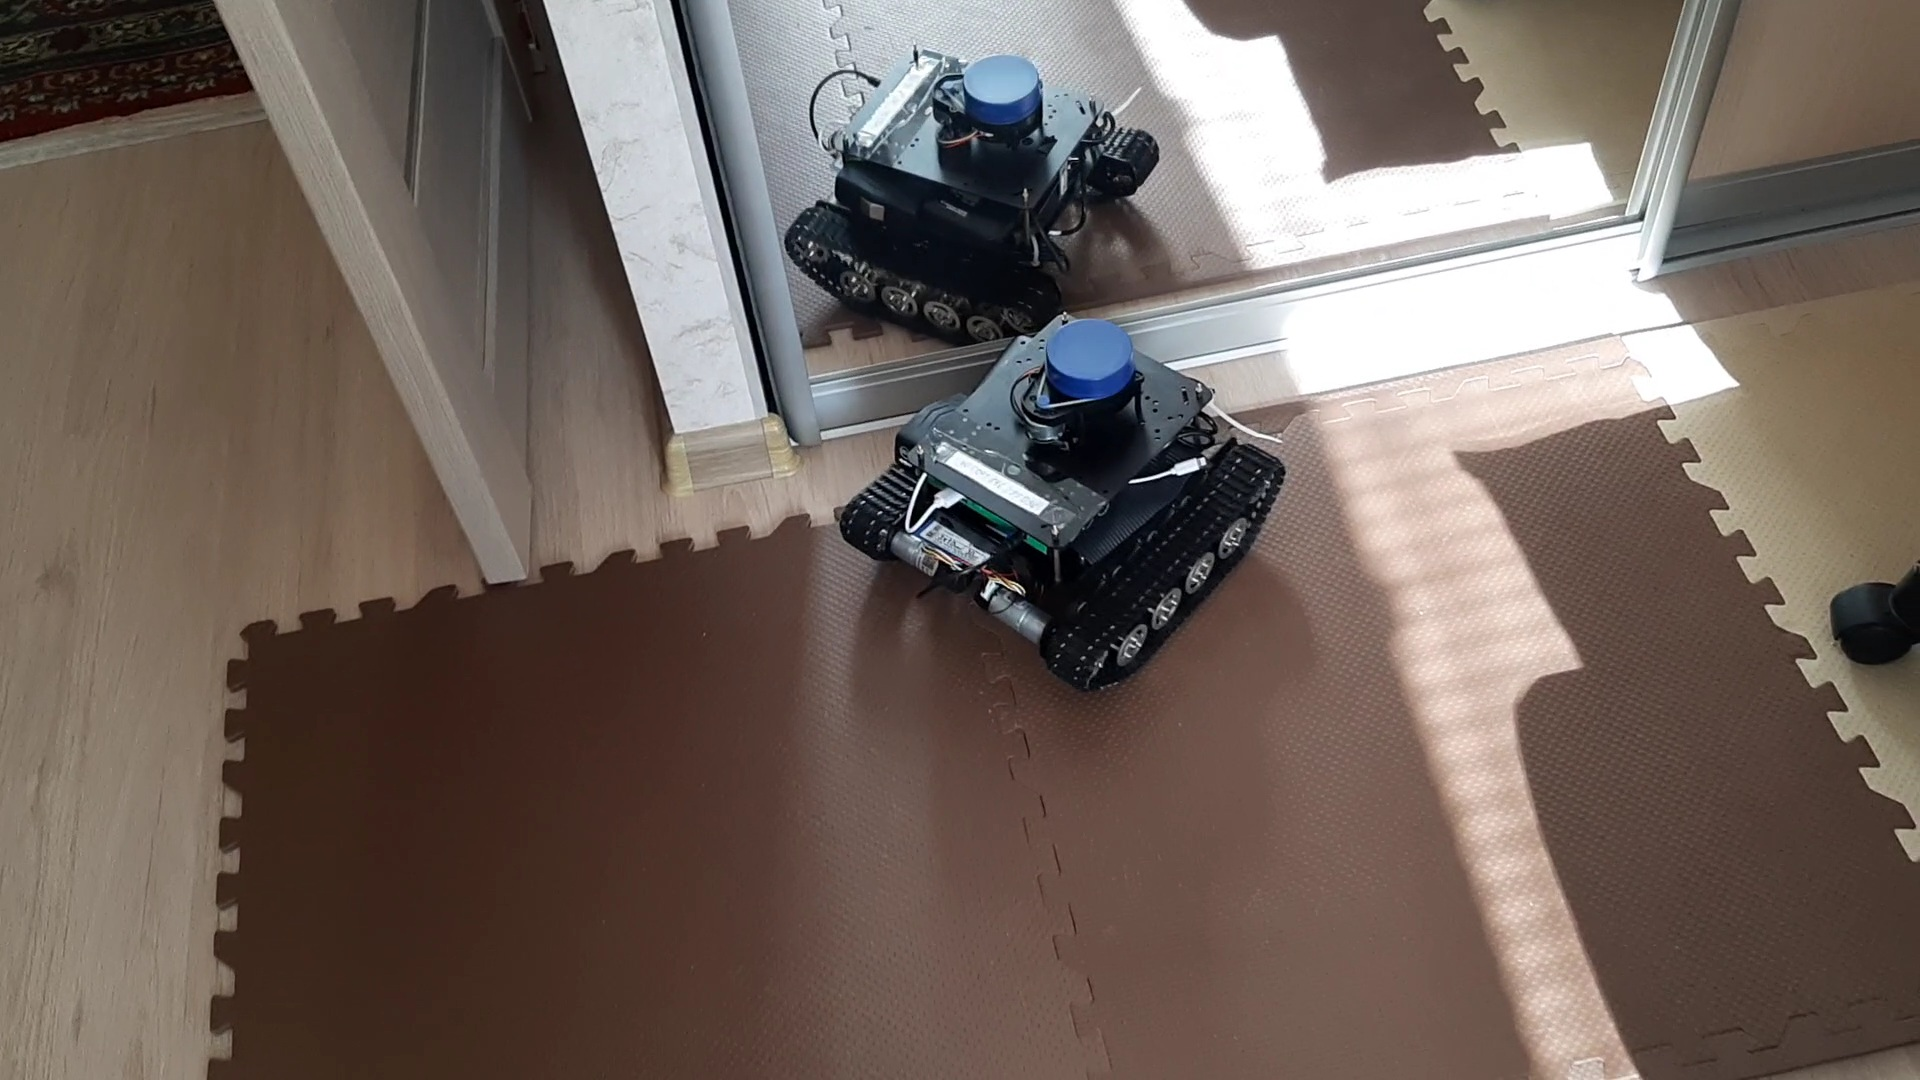
\includegraphics[width=0.5\linewidth]{robot-complete1.jpg} \\
  \end{minipage}
  \hfill
  \begin{minipage}[b][][b]{0.49\linewidth}\centering
    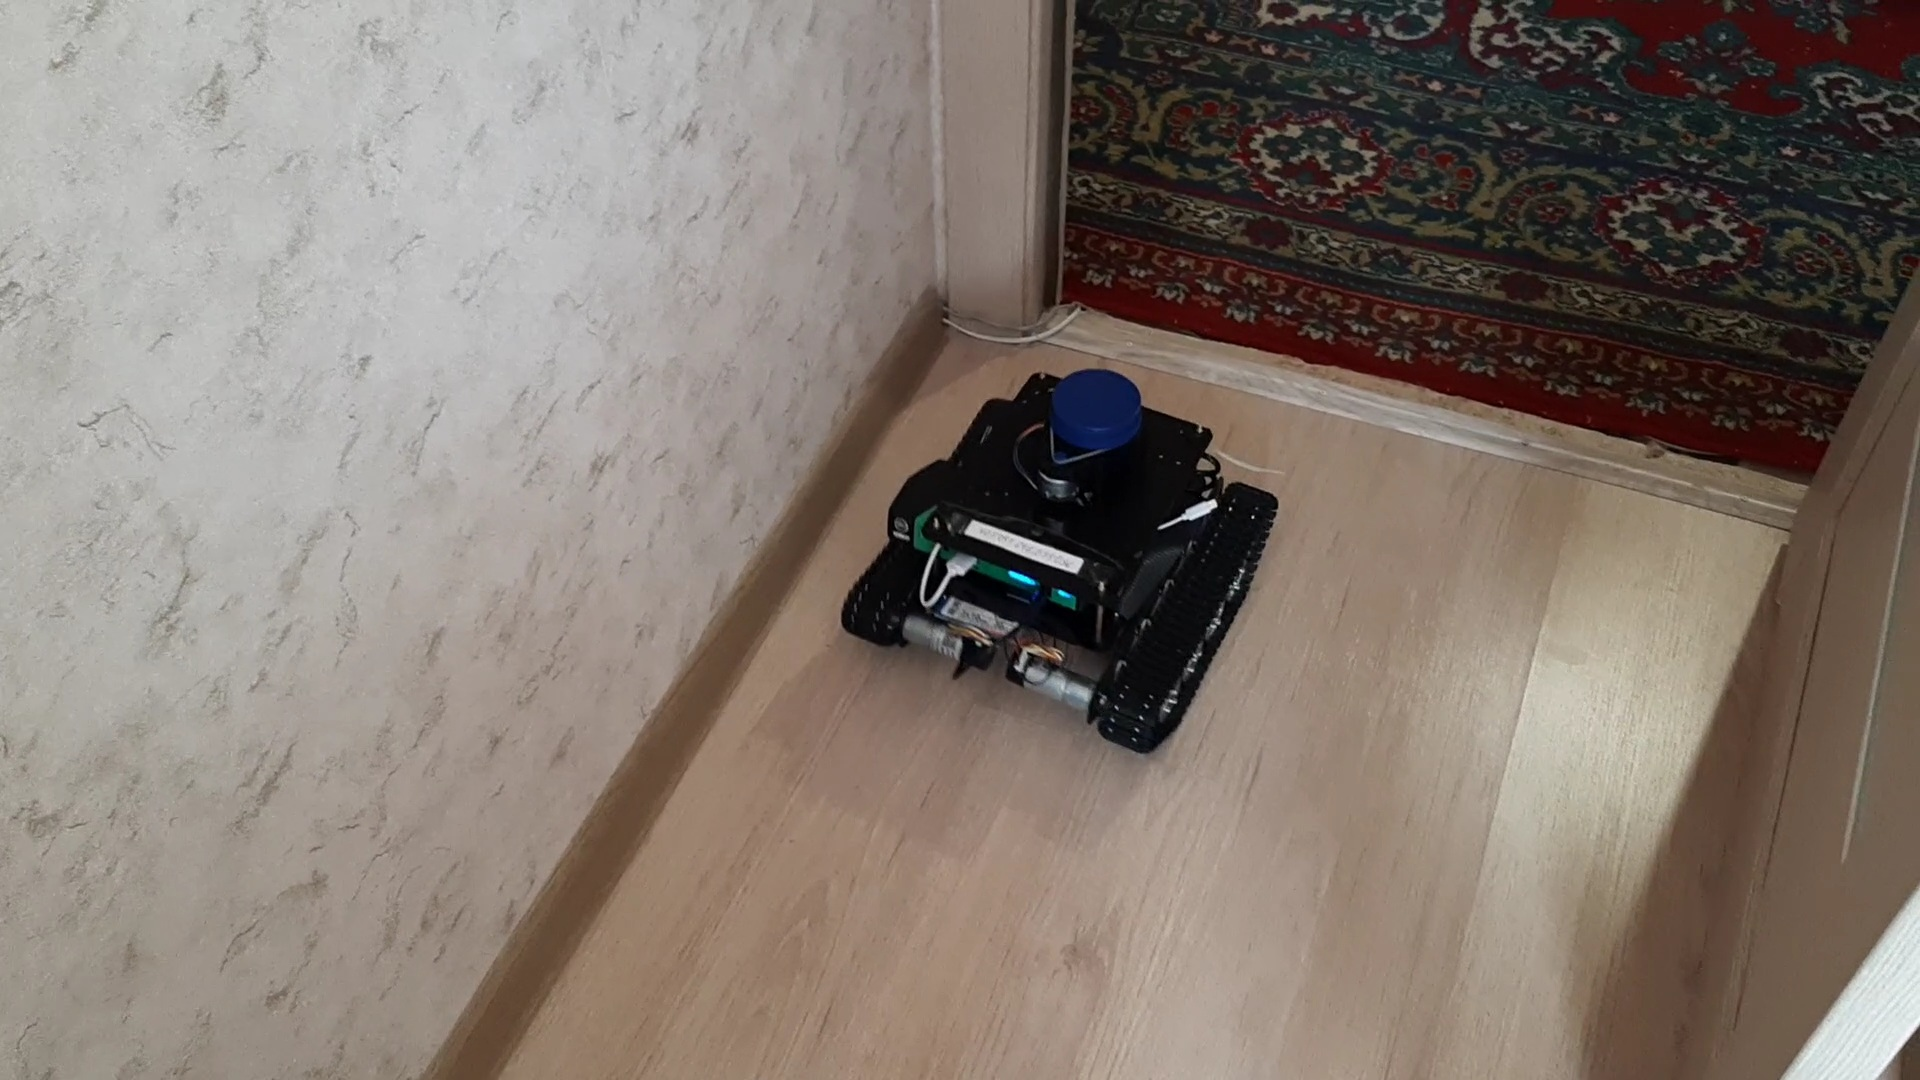
\includegraphics[width=0.5\linewidth]{robot-complete2.jpg} \\
  \end{minipage}
  \hfill
  \begin{minipage}[b][][b]{0.49\linewidth}\centering
    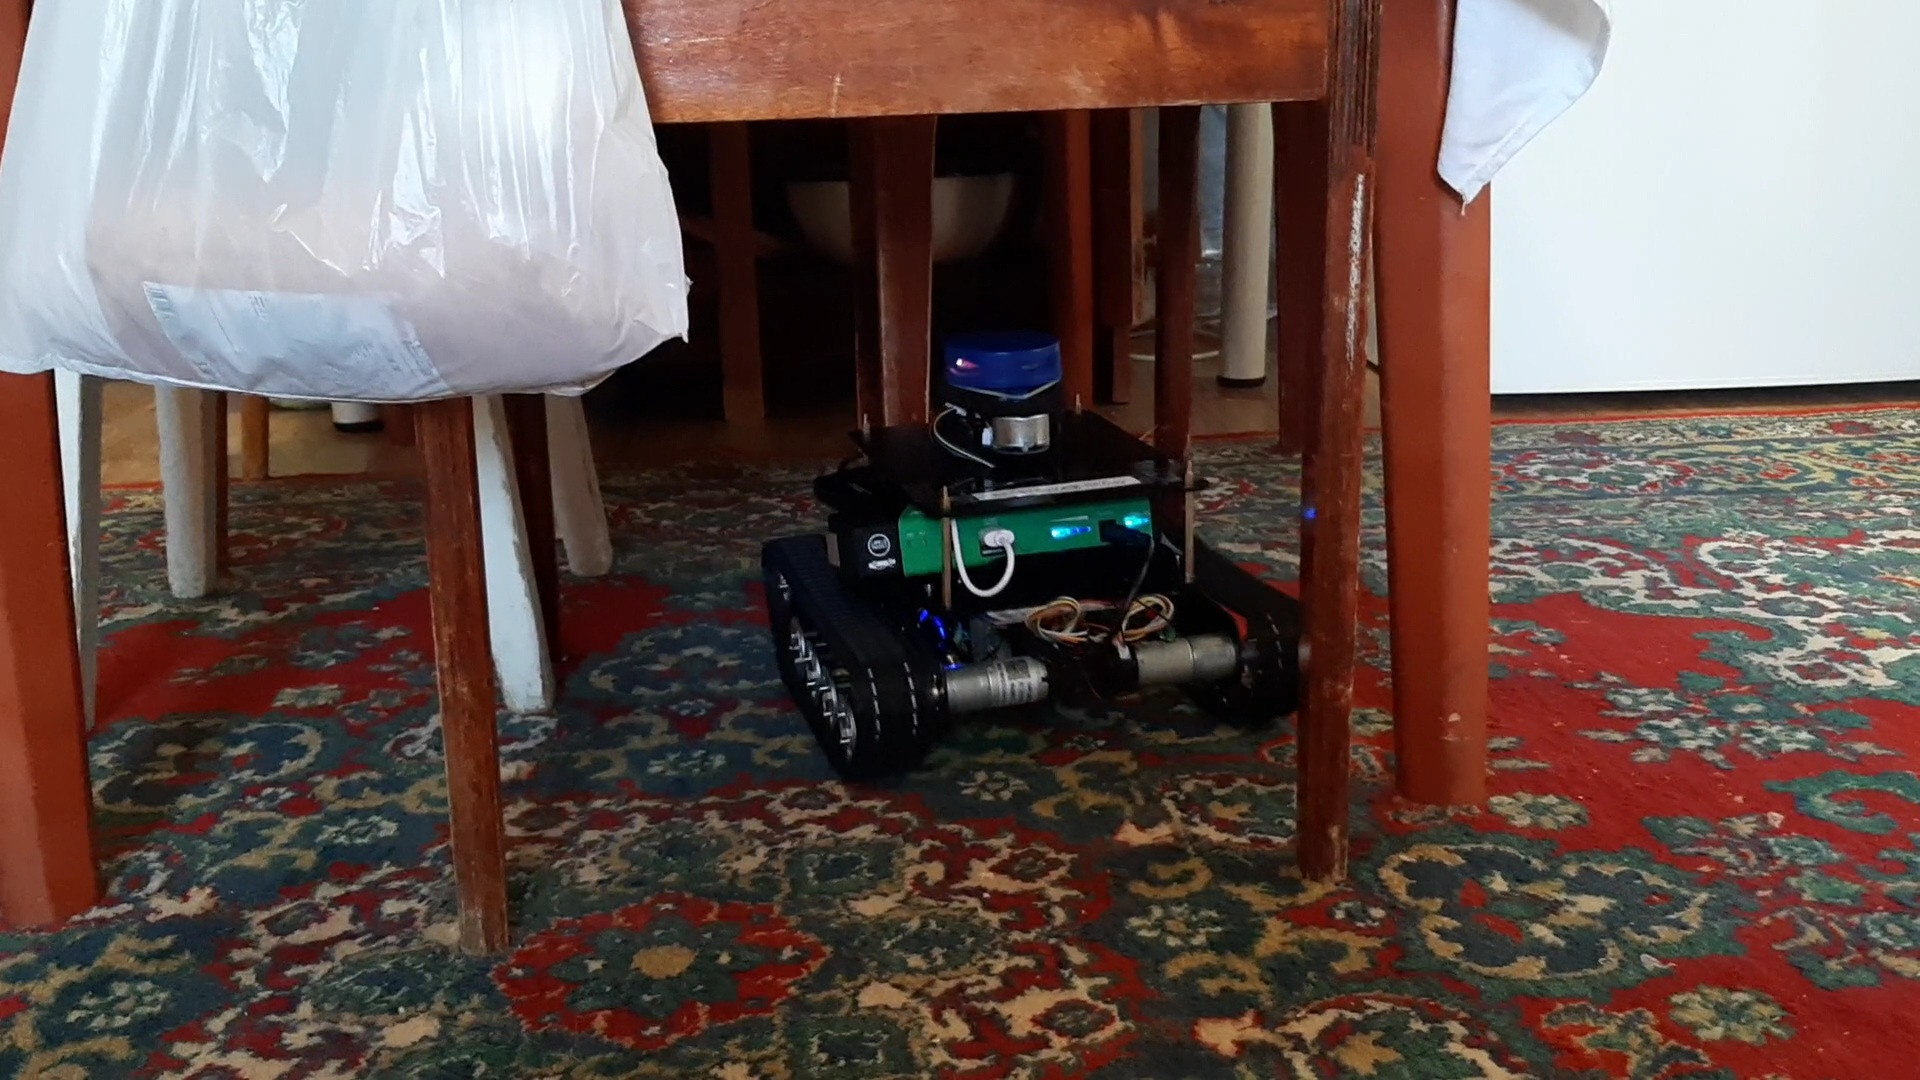
\includegraphics[width=0.5\linewidth]{robot-complete3.jpg} \\
  \end{minipage}
  \caption{Робот }
  \label{fig:knuth}
\end{figure}